% !TEX root = ../main.tex
\chapter{Noise analysis of PSR~J1640+2224} \label{chpt:risultati}

\section{Real data} \label{sec:reali}

\subsection{Validation of Discovery} \label{sec:validazione}

All the analyses of this thesis are performed with \textsc{Discovery}. Since
it is a recent code, we first verify that it reproduces the results of
\textsc{Enterprise}, the reference software introduced in
Section~\ref{sec:software}. We analyze the DR2low data of PSR~J1640+2224
with both codes, using the reference noise model of Section~\ref{NM}, the
priors of Section~\ref{sec:bayes} and the same sampler, so that the only
difference is the implementation of the likelihood.

The posterior distributions are compared in
Figure~\ref{fig:disc_vs_ent}. The contours obtained with the two codes
overlap in all the panels, and so do the one-dimensional posteriors on the
diagonal. The parameter estimates are also in agreement. For example, the
amplitude of the intrinsic red noise is
$\log_{10}A_{\rm RN} = -13.24^{+0.09}_{-0.10}$ with both codes (here and in
the following we quote the median and the $68\%$ credible interval).
The largest difference is found for the spectral index of the DM variations,
$\gamma_{\rm DM} = 4.12^{+2.33}_{-2.28}$ with \textsc{Discovery} and
$\gamma_{\rm DM} = 3.94^{+2.48}_{-2.12}$ with \textsc{Enterprise}, and it is
much smaller than the width of the posterior. The effective number of
samples of Eq.~\eqref{eq:neff} is $1141$ for the \textsc{Discovery} chain and
$1557$ for the \textsc{Enterprise} one, so differences of this size are
expected from the finite length of the chains.

We conclude that \textsc{Discovery} reproduces the results of
\textsc{Enterprise} for this model, and we use it for all the following
analyses.

\begin{figure}[H]
    \centering
    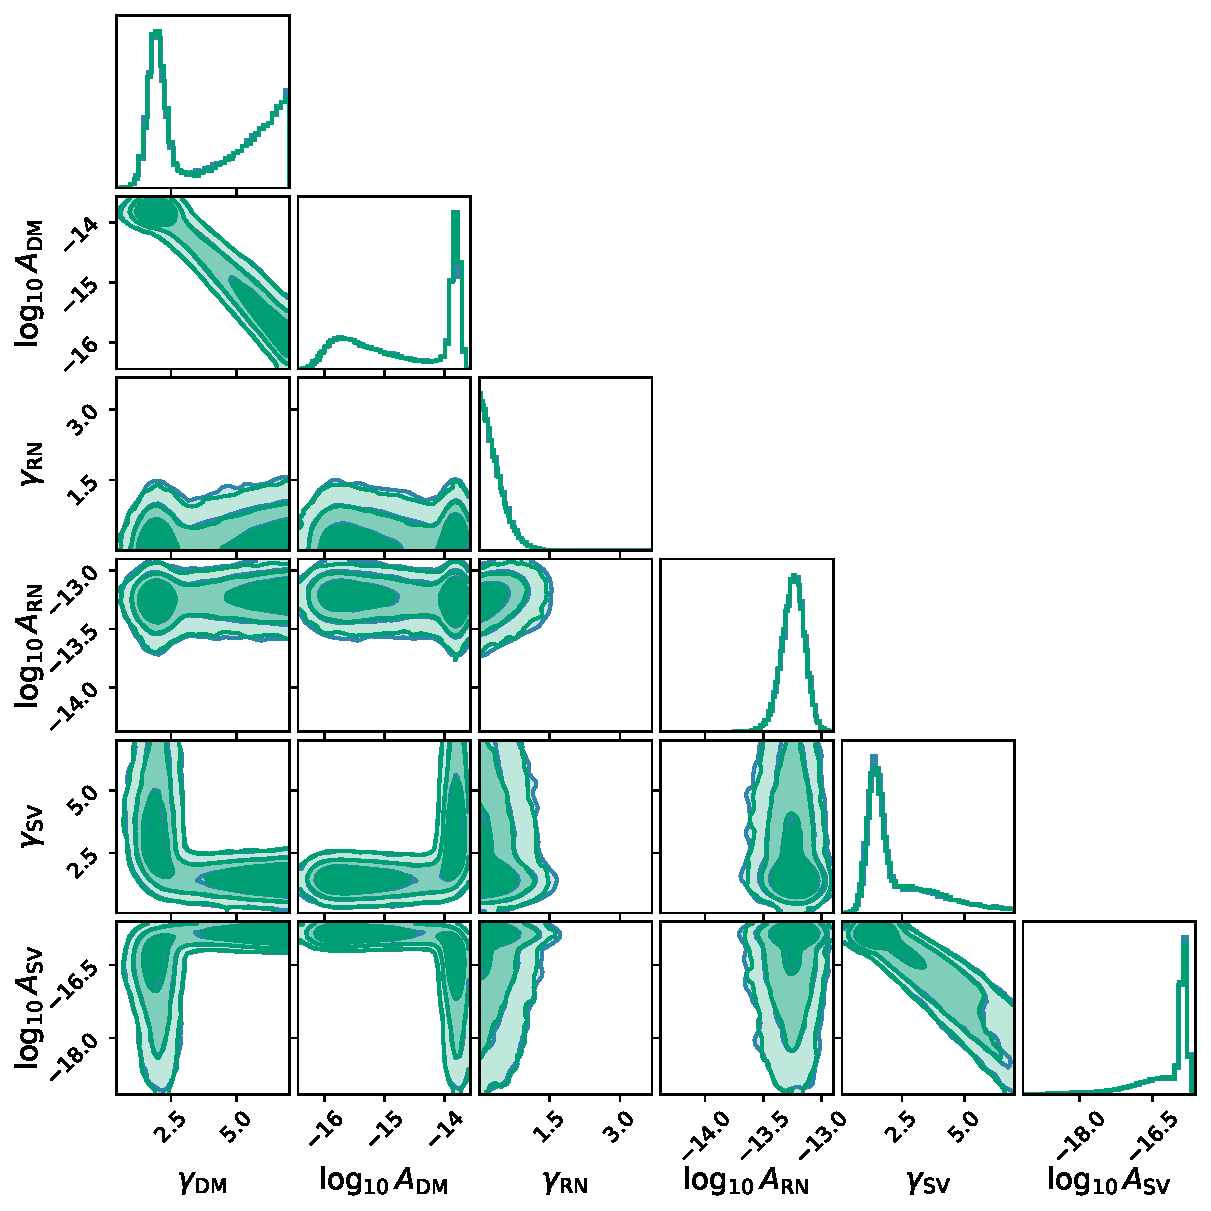
\includegraphics[width=\textwidth]{Figure/cap5/01_discovery_vs_enterprise.pdf}
    \caption{Posterior distributions of the six noise parameters of
    PSR~J1640+2224 obtained from the DR2low data with \textsc{Discovery}
    (blue) and with \textsc{Enterprise} (green). The contours enclose $68\%$,
    $95\%$ and $99.7\%$ of the probability.}
    \label{fig:disc_vs_ent}
\end{figure}

\subsection{DR2low and DR2new+} \label{sec:dr2new}

To show the role of the low radio frequencies, we repeat the analysis on
the DR2new+ dataset, which contains only the observations of the EPTA
telescopes at 1.3--2.6\,GHz, without the LOFAR data. For PSR~J1640+2224 it
consists of $1546$ TOAs over a time span of $10.2$\,yr, against the $6777$
TOAs over $12.2$\,yr of DR2low. The noise model, the number of Fourier
components and the priors are the same used for DR2low.

The two posterior distributions are compared in
Figure~\ref{fig:dr2low_vs_dr2new}. With DR2new+ none of the parameters of
the chromatic processes is constrained. The posteriors of
$\gamma_{\rm DM}$ and $\gamma_{\rm SV}$ cover the whole prior range, and
those of the amplitudes extend from the lower bound of the prior up to
$\log_{10}A \simeq -13$, so that the data only exclude the largest
amplitudes. The same happens for the intrinsic red noise. In the band of
DR2new+ the chromatic factor of Eq.~\eqref{eq:chrom} is close to one, so
the three processes have almost the same effect on the timing residuals
and the data cannot tell which of them is present.

With DR2low the posteriors are much narrower. The LOFAR observations are
at radio frequencies about ten times lower, where the DM variations and
the scattering variations are much stronger and depend on $\nu$ in
different ways, and this allows the chromatic processes to be separated
from the achromatic red noise. The amplitude of the intrinsic red noise,
for example, is unconstrained with DR2new+, while with DR2low it is
$\log_{10}A_{\rm RN} = -13.24^{+0.09}_{-0.10}$. A good coverage in radio
frequency is therefore necessary to measure the chromatic noise of this
pulsar.

\begin{figure}[H]
    \centering
    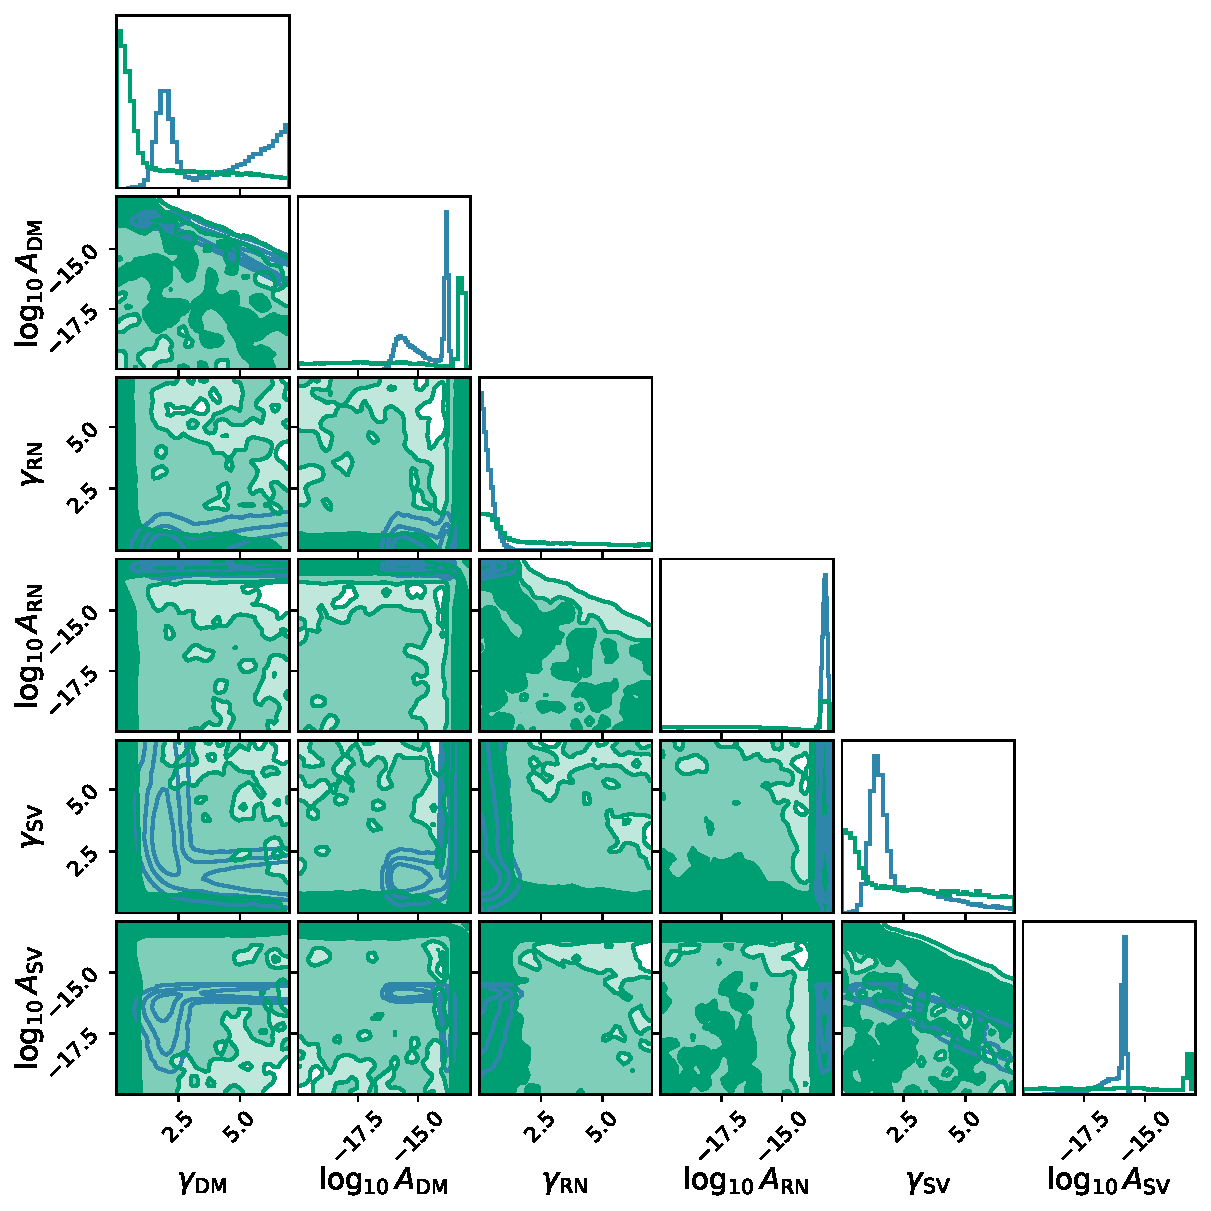
\includegraphics[width=\textwidth]{Figure/cap5/02_DR2low_vs_DR2newplus.pdf}
    \caption{Posterior distributions of the six noise parameters of
    PSR~J1640+2224 obtained from the DR2low data (blue) and from the DR2new+
    data (green). The contours enclose $68\%$, $95\%$ and $99.7\%$ of the
    probability. The axes cover the full range of the priors.}
    \label{fig:dr2low_vs_dr2new}
\end{figure}